
\noindent\begin{minipage}{\textwidth}
    \begin{table}[H]
        \centering
        \caption{Hiperparâmetros e Resultados do Melhor Modelo - resnet\_v9\_AM\_opt\_aug}
        \vspace{0.2cm}
        \resizebox{\textwidth}{!}{%
            \begin{tabular}{ll | lrrr}
                \hline
                \multicolumn{2}{c|}{\textbf{Hiperparâmetros}} & \multicolumn{4}{c}{\textbf{Métricas por Classe}} \\ \hline
                \textbf{Parâmetro} & \textbf{Valor} & \textbf{Classe} & \textbf{Precisão} & \textbf{Recall} & \textbf{F1-Score} \\ \hline
    Agendador de LR & StepLR & 31.2 & 0.5019 & 0.5841 & 0.5399 \\ 
Architecture & resnet50 & 31.3 & 0.3878 & 0.5050 & 0.4387 \\ 
Augmentation (Método) & None & 31.4 & 0.3897 & 0.5048 & 0.4398 \\ 
Batch Size & 32 & 32.3 & 0.6863 & 0.3571 & 0.4698 \\ 
Decaimento de Peso (WD) & 0.0001 & 32.4 & 0.3968 & 0.4310 & 0.4132 \\ 
Dropout & 0.3430 & 33.3 & 0.5556 & 0.3627 & 0.4389 \\ 
Função de Perda & CrossEntropyLoss & 41.4 & 0.4000 & 0.2727 & 0.3243 \\ 
Hidden Units & 512 & 41.5 & 0.6000 & 0.5385 & 0.5676 \\ 
Label Smoothing & 0.1000 & 42.4 & 0.4565 & 0.6176 & 0.5250 \\ 
Otimizador & AdamW & 44.4 & 0.7895 & 0.5172 & 0.6250 \\ 
\cline{3-6} 
Taxa de Aprendizado (LR) & 1.81e-04 & \textbf{Média (Macro)} & 0.5164 & 0.4691 & 0.4782 \\ 
Unfreeze Layers & 3 & \textbf{MCC} & \multicolumn{3}{c}{0.3860} \\ 
            \hline
            \end{tabular}%
        }
    \end{table}

    \begin{figure}[H]
        \centering
        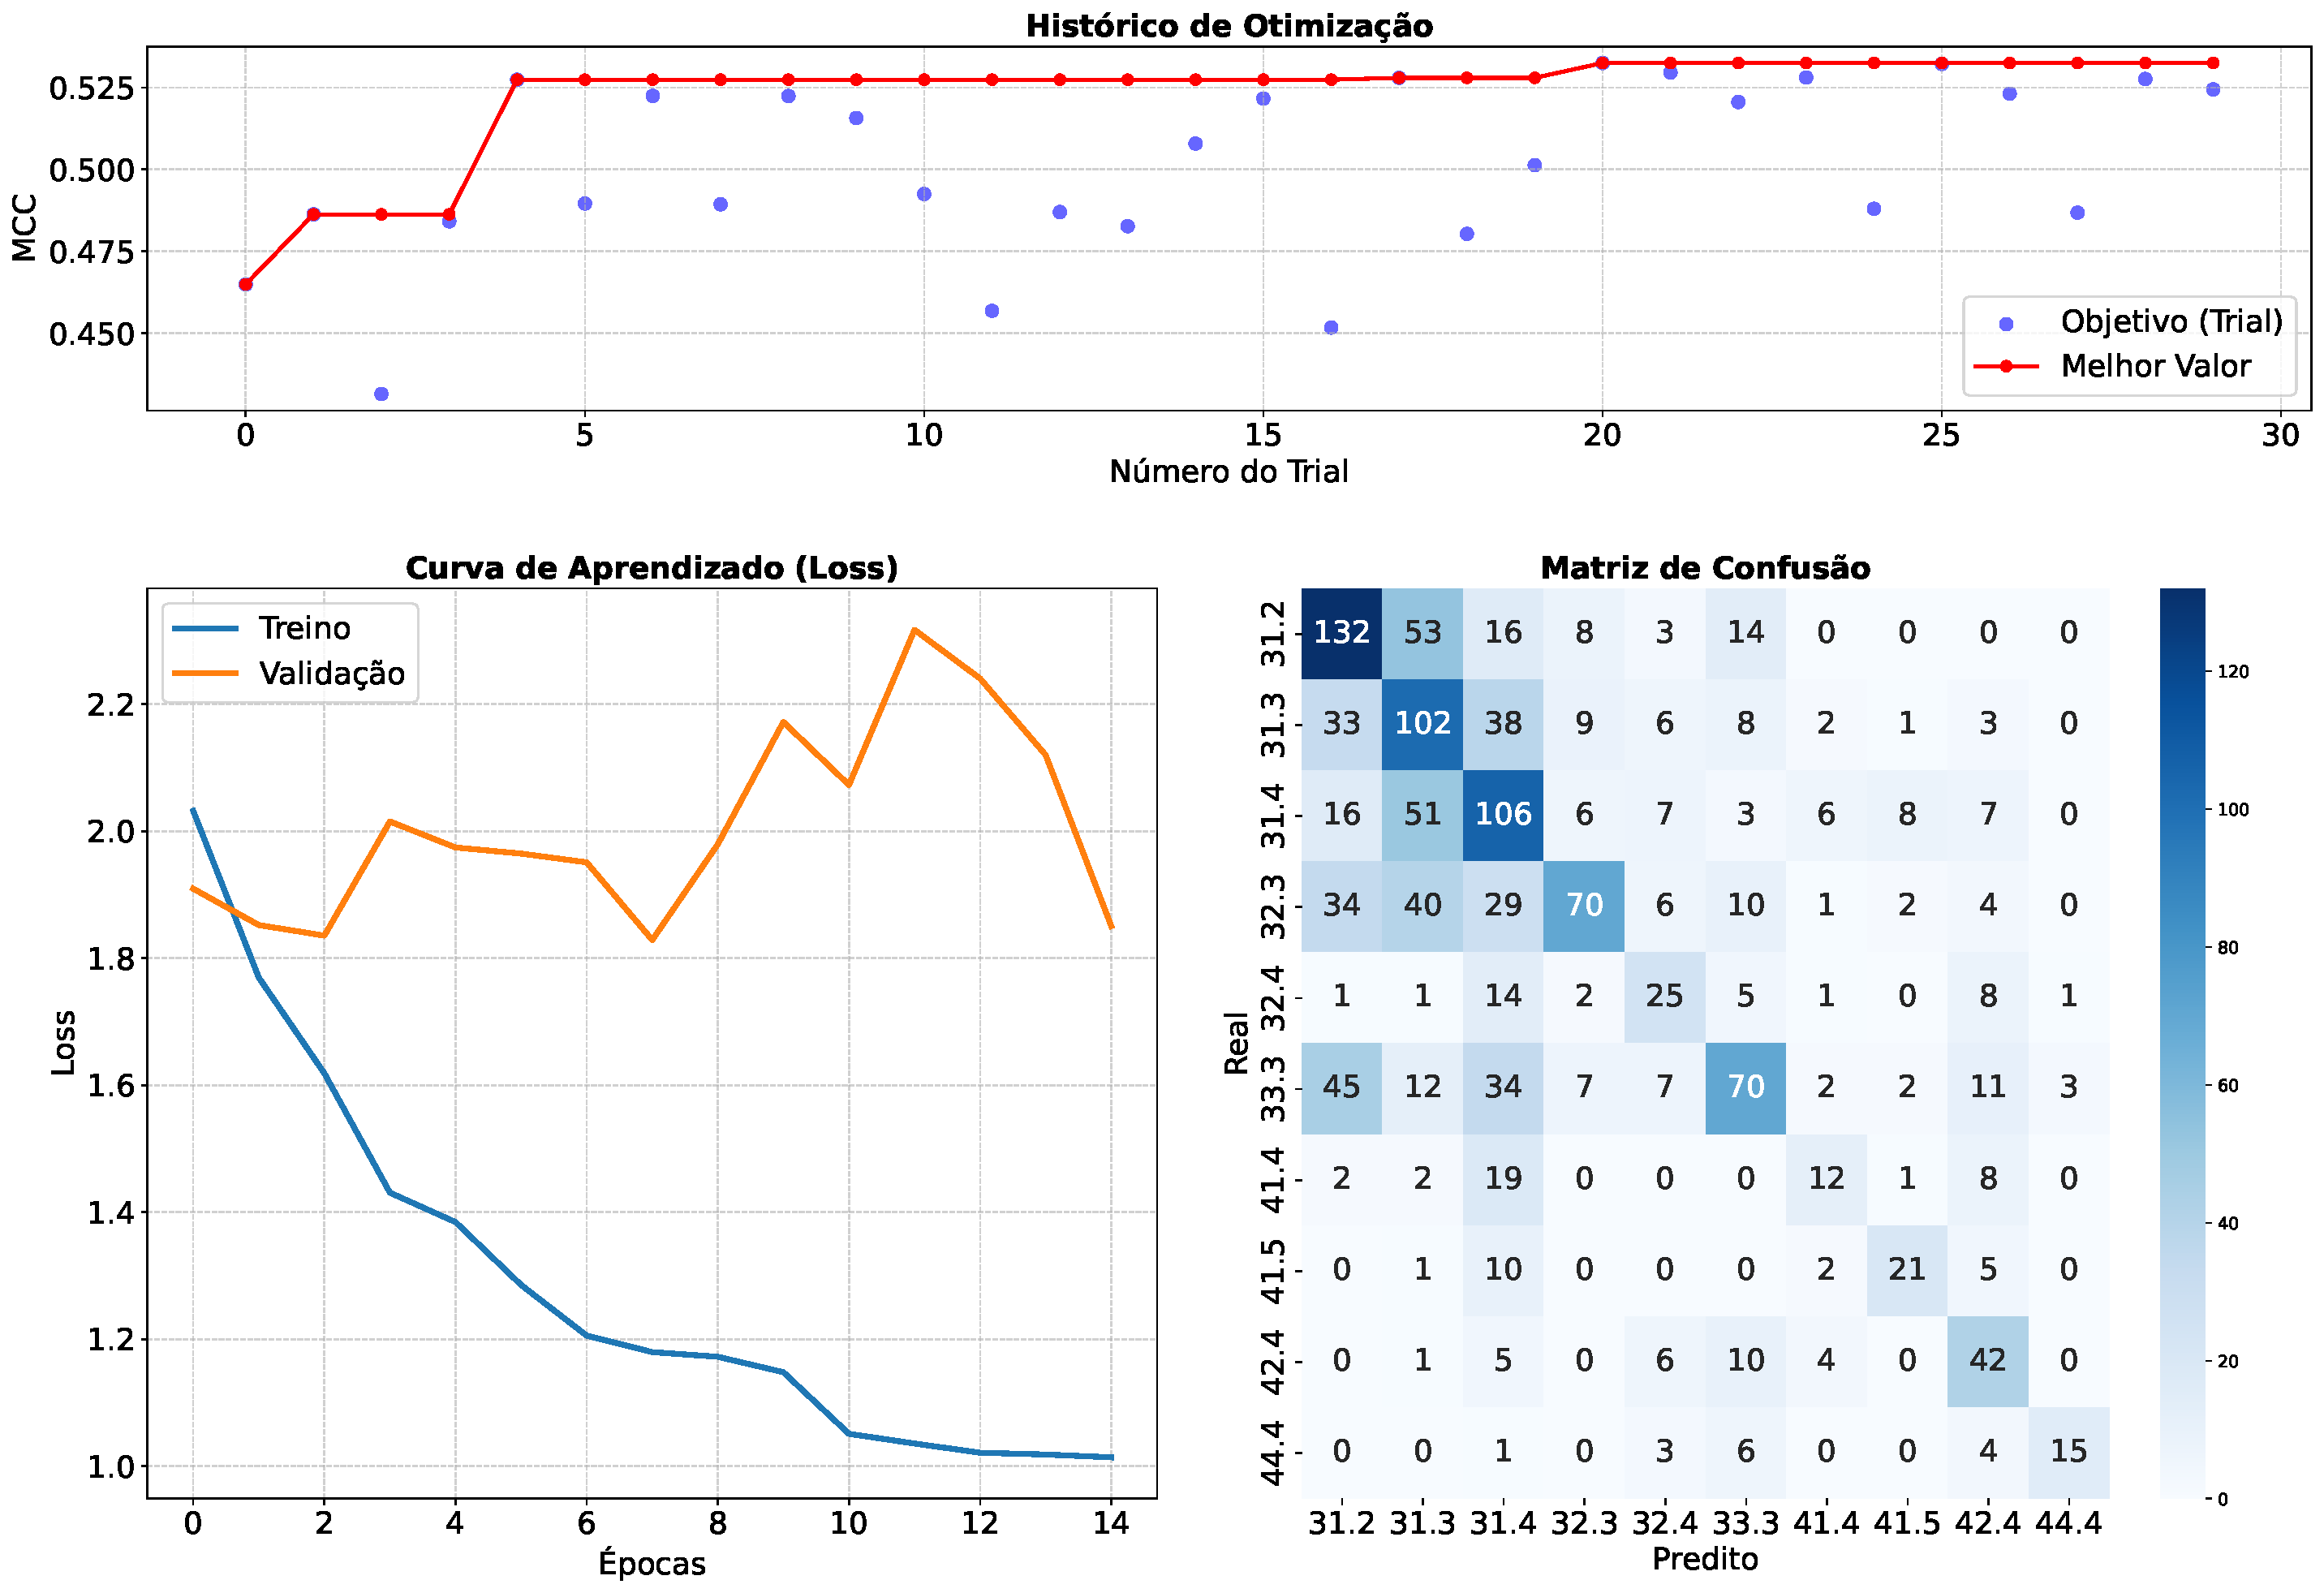
\includegraphics[width=0.85\textwidth]{tex/appendix/experiments/resnet_v9_AM_opt_aug/dashboard_consolidado.pdf}
        \caption{Histórico de Otimização, Curvas de Aprendizado e Matriz de Confusão - resnet\_v9\_AM\_opt\_aug}
    \end{figure}
\end{minipage}
\clearpage
